\section{Case Studies}
\label{surface_reconstruction_section_case_studies}

The surface reconstruction problem being inherently ill-posed, the proposed algorithm does not pretend to reconstruct all kinds of surfaces with arbitrary sampling conditions. This section provides the user with some hints about the ideal sampling and contouring conditions, and depicts some failure cases when these conditions are not matched.

\subsection{Ideal Conditions}

The user must keep in mind that the poisson surface reconstruction algorithm comprises two phases (computing the implicit function from the input point set and contouring an iso-surface of this function). Both require some care in terms of sampling conditions and parameter tuning.

\subsubsection{Point Set}

Ideally the current implementation of the Poisson surface reconstruction method expects a dense 3D oriented point set (typically matching the epsilon-sampling condition~\cite{cgal:bo-pgsms-05}) and sampled over a closed, smooth surface. Oriented herein means that all 3D points must come with consistently oriented normals to the inferred surface. Figures \ref{Surface_reconstruction_points_3-fig-bimba} and \ref{Surface_reconstruction_points_3-fig-eros} illustrate cases where these ideal conditions are met.

% Insert image bimba.jpg/.eps
\begin{center}
    \begin{ccTexOnly}
        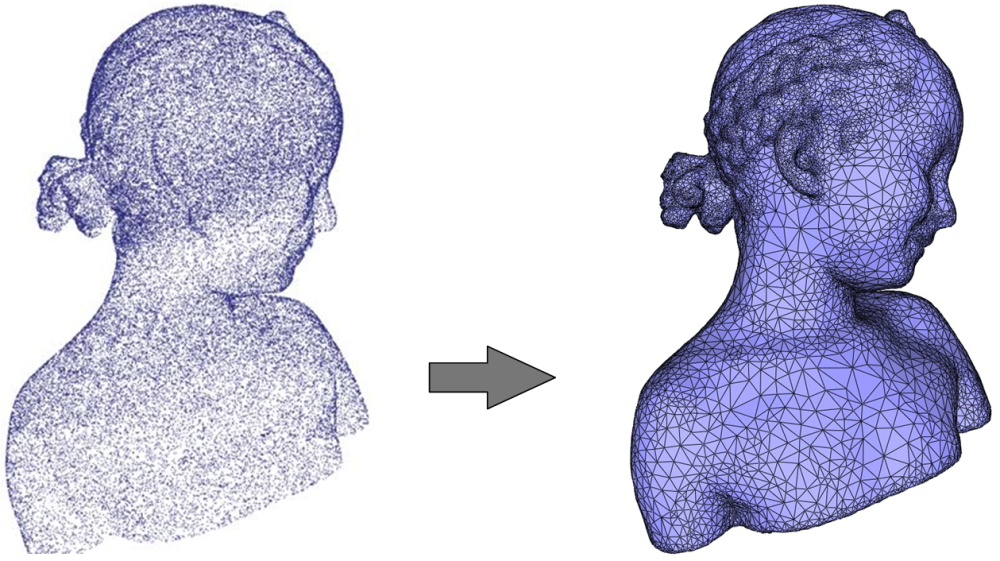
\includegraphics[width=1.0\textwidth]{Surface_reconstruction_points_3/bimba}
    \end{ccTexOnly}
    \begin{ccHtmlOnly}
        <img style="max-width: 80%;" border=0 src="./bimba.jpg"><P>
    \end{ccHtmlOnly}
    \begin{figure}[h]
        \caption{Poisson reconstruction.
                 Left: 120K points sampled on a statue (Minolta laser scanner).
                 Right: reconstructed surface mesh.}
        \label{Surface_reconstruction_points_3-fig-bimba}
    \end{figure}
\end{center}

% Insert image eros.jpg/.eps
\begin{center}
    \begin{ccTexOnly}
        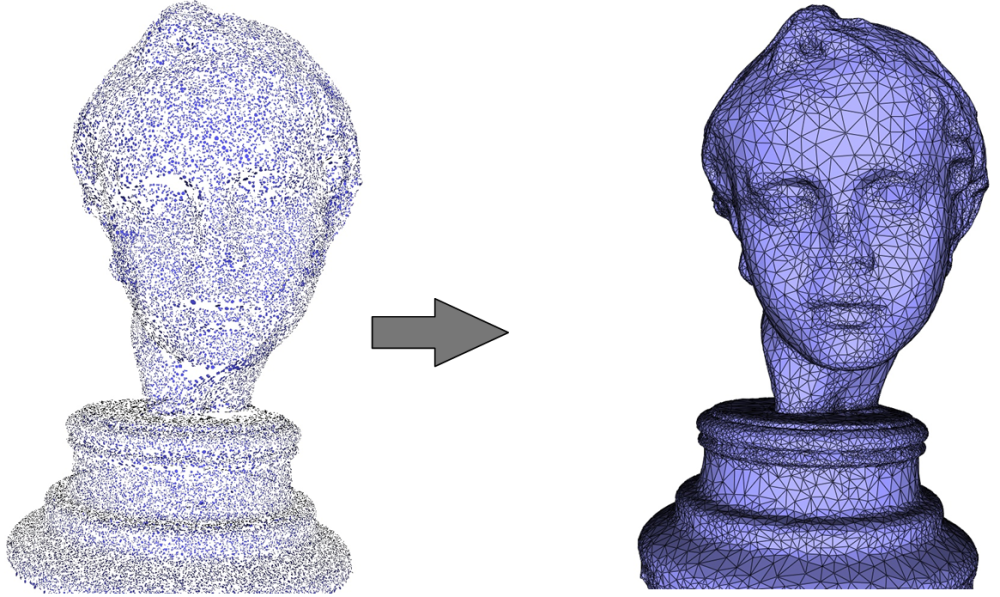
\includegraphics[width=1.0\textwidth]{Surface_reconstruction_points_3/eros}
    \end{ccTexOnly}
    \begin{ccHtmlOnly}
        <img style="max-width: 80%;" border=0 src="./eros.jpg"><P>
    \end{ccHtmlOnly}
    \begin{figure}[h]
        \caption{Left: 120K points sampled on a statue (Minolta laser scanner).
                 Right: reconstructed surface mesh.}
        \label{Surface_reconstruction_points_3-fig-eros}
    \end{figure}
\end{center}

The algorithm is fairly robust to anisotropic sampling and to noise. It is also robust to missing data through filling the corresponding holes as the algorithm is designed to reconstruct the indicator function of an inferred solid (see Figure~\ref{Surface_reconstruction_points_3-fig-holes_good}).

% Insert image holes_good.jpg/.eps
\begin{center}
    \begin{ccTexOnly}
        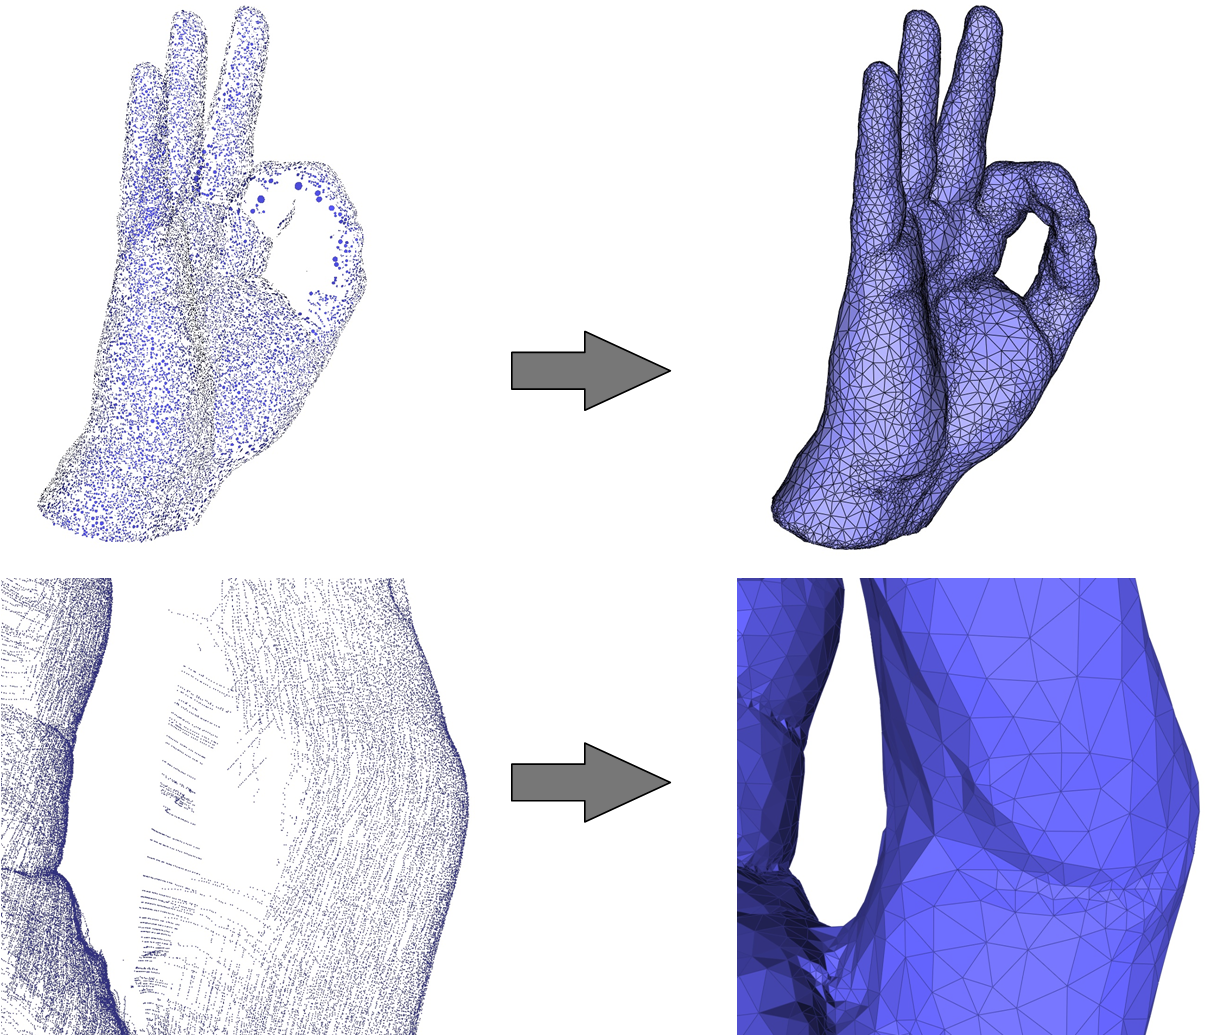
\includegraphics[width=1.0\textwidth]{Surface_reconstruction_points_3/holes_good} % omit .eps suffix
    \end{ccTexOnly}
    \begin{ccHtmlOnly}
        <img style="max-width: 80%;" border=0 src="./holes_good.jpg"><P>
    \end{ccHtmlOnly}
    \begin{figure}[h]
        \caption{Top left: 65K points sampled on a hand (Kreon laser scanner).
                 Bottom left: the point set is highly anisotropic due
                 to the scanning technology.
                 Right: reconstructed surface mesh and closeup.
                 The holes are properly closed.}
        \label{Surface_reconstruction_points_3-fig-holes_good}
    \end{figure}
\end{center}

The algorithm is in general not robust to outliers, although a few outliers do not always create a failure, see Figure~\ref{Surface_reconstruction_points_3-fig-outliers}.

% Insert image outliers.jpg/.eps
\begin{center}
    \begin{ccTexOnly}
        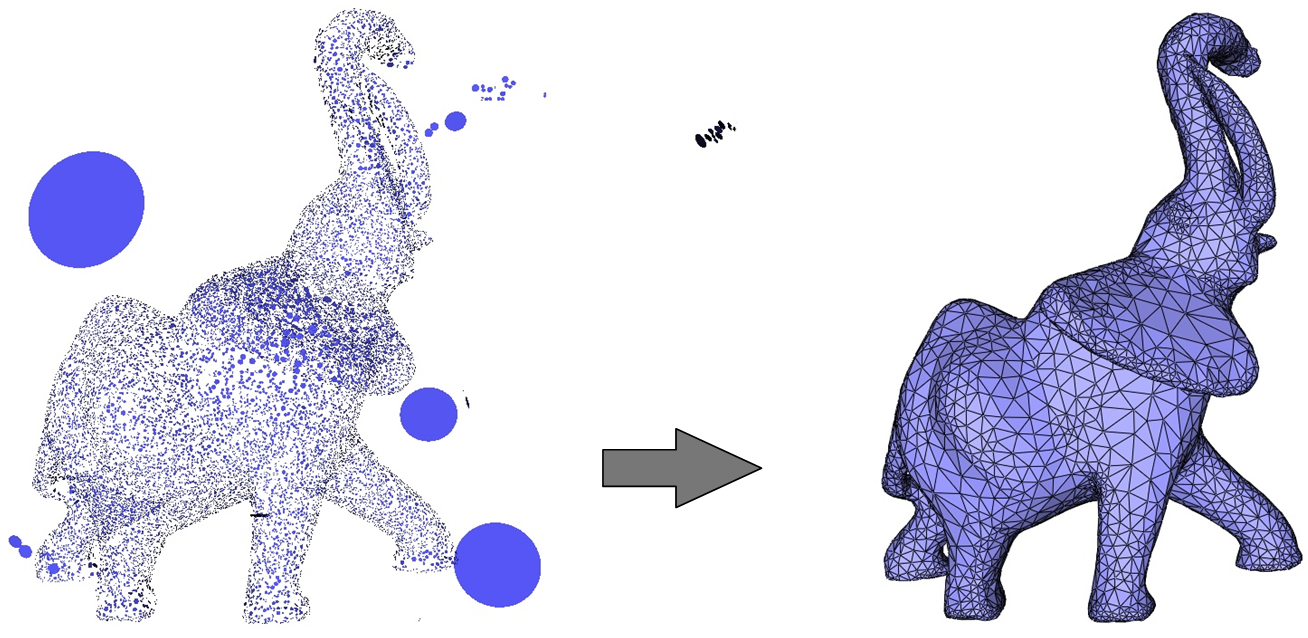
\includegraphics[width=1.0\textwidth]{Surface_reconstruction_points_3/outliers} % omit .eps suffix
    \end{ccTexOnly}
    \begin{ccHtmlOnly}
        <img style="max-width: 80%;" border=0 src="./outliers.jpg"><P>
    \end{ccHtmlOnly}
    \begin{figure}[h]
        \caption{Left: 70K points sampled on an elephant with few
                 outliers emphasized with disks.
                 Right: reconstructed surface mesh.}
        \label{Surface_reconstruction_points_3-fig-outliers}
    \end{figure}
\end{center}


The algorithm works well even when the inferred surface is composed of several connected components, provided that both all normals are properly estimated and oriented (the current \cgal\ normal orienter algorithm may fail in some cases, see \ccc{CGAL::mst_orient_normals()}), and that the final contouring algorithm is properly seeded for each component. When the inferred surface is composed of several nested connected components care should be taken to orient the normals of each component in alternation (inward/outward) so that the final contouring stage picks a proper contouring value.


\subsubsection{Contouring Parameters}

Our implementation of the Poisson surface reconstruction algorithm computes an implicit function represented as a piecewise linear function over the tetrahedra of a 3D Delaunay triangulation constructed from the input points then refined through Delaunay refinement. For this reason, any iso-surface is also piecewise linear and hence may contain sharp creases. As the contouring algorithm \ccc{CGAL::make_surface_mesh()} expects a smooth implicit function these sharp creases may create spurious clusters of vertices in the final reconstructed surface mesh when setting a small mesh sizing or surface approximation error parameter (see Figure~\ref{Surface_reconstruction_points_3-fig-contouring_bad}).\\
One way to avoid these spurious clusters consists of adjusting the mesh sizing and surface approximation parameters large enough compared to the average sampling density (obtained through \ccc{CGAL::compute_average_spacing()}) so that the contouring algorithm ``perceives'' a smooth iso-surface. We recommend to use the following contouring parameters:
\begin{itemize}
\item Max triangle radius: at least 100 times the average spacing.
\item Approximation distance: at least 0.25 times the average spacing.
\end{itemize}

% PA: we are missing the number of input points here.
% Insert image contouring_bad.jpg/.eps
\begin{center}
    \begin{ccTexOnly}
        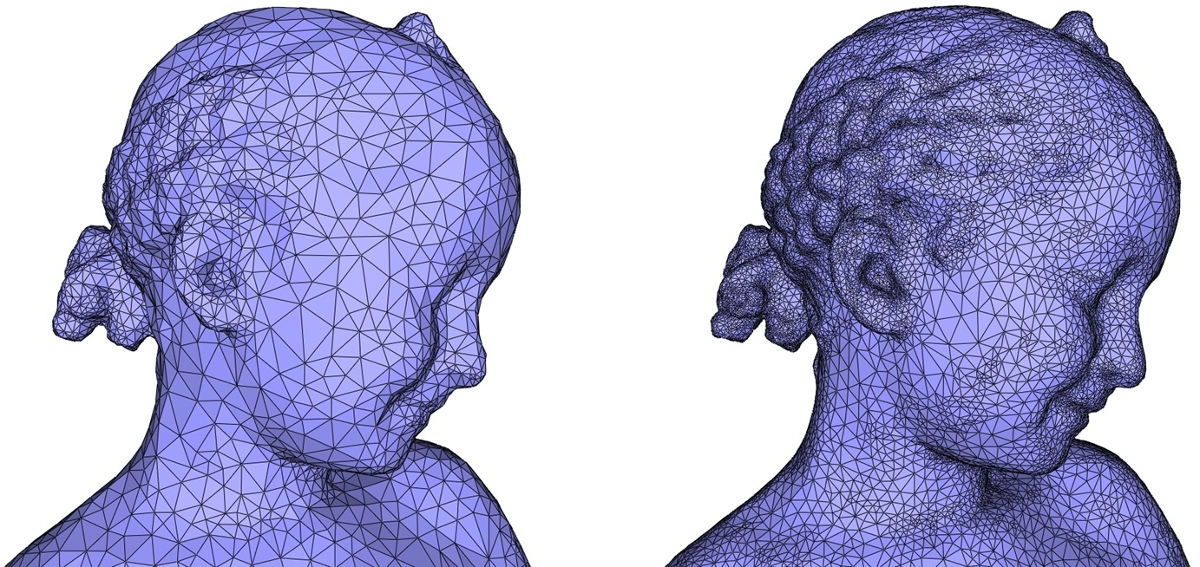
\includegraphics[width=1.0\textwidth]{Surface_reconstruction_points_3/contouring_bad}
    \end{ccTexOnly}
    \begin{ccHtmlOnly}
        <img style="max-width: 80%;" border=0 src="./contouring_bad.jpg"><P>
    \end{ccHtmlOnly}
    \begin{figure}[h]
        \caption{Left: surface reconstructed with approximation
                 distance = 0.25 * average spacing.
                 Right: surface reconstructed with approximation
                 distance = 0.15 * average spacing.
                 Notice the spurious cluster on the chick.}
        \label{Surface_reconstruction_points_3-fig-contouring_bad}
    \end{figure}
\end{center}


\subsection{Degraded Conditions}

The conditions listed above are rather restrictive and in practice not all of them are met in the applications. We now illustrates the behavior of the algorithm when the conditions are not met in terms of sampling, wrongly oriented normals, noise and sharp creases.

\subsubsection{Sparse Sampling}

The reconstruction algorithm expects a sufficiently dense point set. Although there is no formal proof of correctness of the algorithm under certain density conditions due to its variational nature, our experiments show that the algorithm reconstructs well all thin features when the local spacing is at most one tenth of the local feature size (the distance to the medial axis, which captures altogether curvature, thickness and separation). When this condition is not met the reconstruction does not reconstruct the thin undersampled features (see Figure~\ref{Surface_reconstruction_points_3-fig-sampling}).

% Insert image sampling.jpg/.eps
\begin{center}
    \begin{ccTexOnly}
        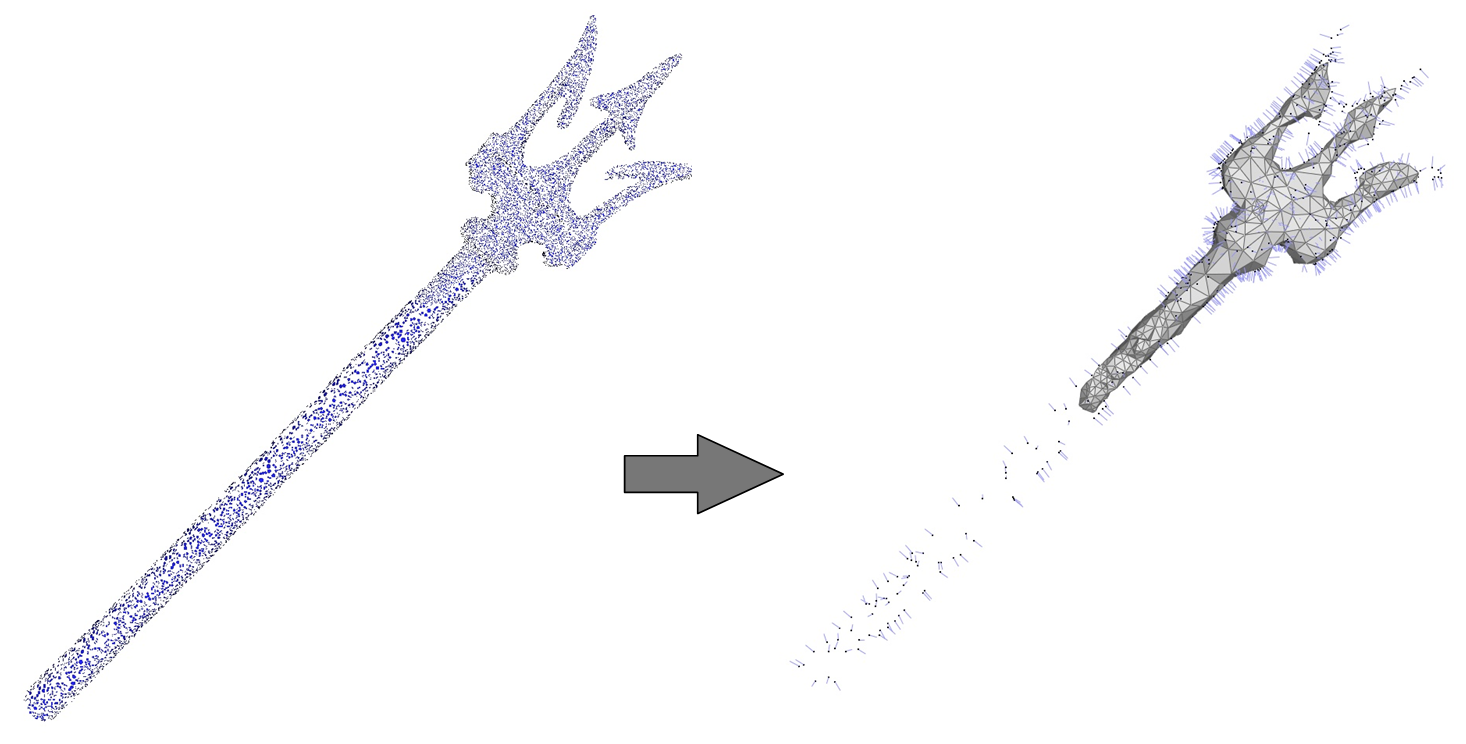
\includegraphics[width=0.8\textwidth]{Surface_reconstruction_points_3/sampling}
    \end{ccTexOnly}
    \begin{ccHtmlOnly}
        <img style="max-width: 80%;" border=0 src="./sampling.jpg"><P>
    \end{ccHtmlOnly}
    \begin{figure}[h]
        \caption{Left: 50K points sampled on the Neptune trident.
                 The reconstruction (not shown) is successful in this case.
                 % PA: better to show it... this may confuse the reader.
                 Right: point set simplified to 1K points then reconstructed
                 (all input points are depicted with normals). The thin
                 feature is not reconstructed.}
        \label{Surface_reconstruction_points_3-fig-sampling}
    \end{figure}
\end{center}


\subsubsection{Large Holes}

The reconstruction is devised to solve for an implicit function which is an approximate indicator function of an inferred solid. For this reason the contouring algorithm always extracts a closed surface mesh and hence is able to fill the small holes where data are missing due, e.g., to occlusions during acquisition. In case of large holes the algorithm still closes them all but sometimes in an unexpected manner. In addition the resulting piecewise linear implicit function may exhibit large triangle patches and sharp creases as the 3D Delaunay triangulation used for solving is very coarse where the holes are filled (see Figure~\ref{Surface_reconstruction_points_3-fig-holes_bad}).

% Insert image holes_bad.jpg/.eps
\begin{center}
    \begin{ccTexOnly}
        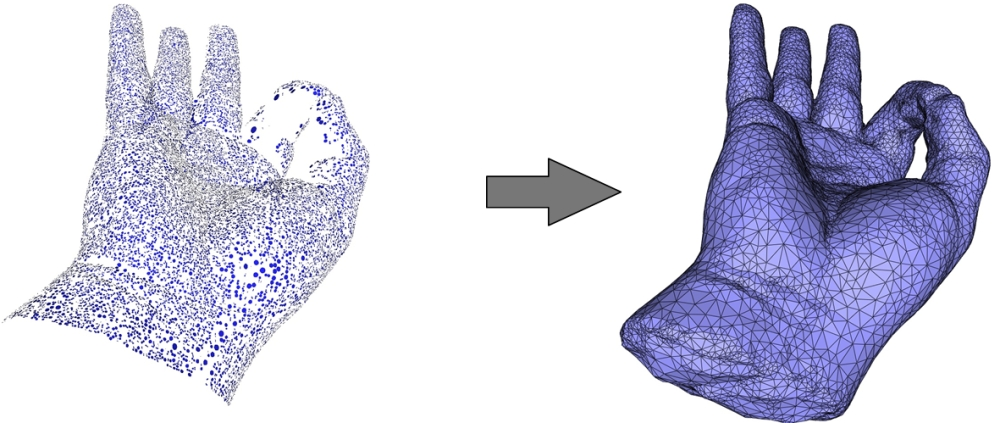
\includegraphics[width=0.8\textwidth]{Surface_reconstruction_points_3/holes_bad}
    \end{ccTexOnly}
    \begin{ccHtmlOnly}
        <img style="max-width: 80%;" border=0 src="./holes_bad.jpg"><P>
    \end{ccHtmlOnly}
    \begin{figure}[h]
        \caption{Left: 65K points sampled on a hand with no data
                 captured at the wrist base.
                 Right: reconstructed surface mesh. The surface is
                 properly closed on the fingers and also closed
                 at the wrist but in a less plausible manner.}
        \label{Surface_reconstruction_points_3-fig-holes_bad}
    \end{figure}
\end{center}


\subsubsection{Wrongly Oriented Normals}

The Poisson surface reconstruction approaches solves for an implicit function whose gradient best matches a set of input normals. Because it solves this problem in the least squares sense, it is robust to few isolated wrongly oriented (flipped) normals. Nevertheless a cluster of wrongly oriented normals leads to an incorrect implicit function and hence to spurious geometric or even topological distortion (see Figure~\ref{Surface_reconstruction_points_3-fig-flipped_normals}).

% Insert image flipped_normals.jpg/.eps
\begin{center}
    \begin{ccTexOnly}
        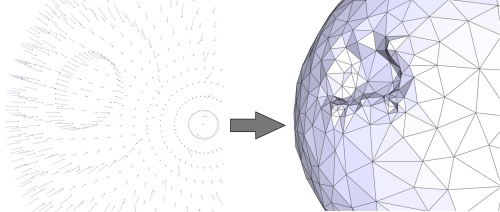
\includegraphics[width=0.8\textwidth]{Surface_reconstruction_points_3/flipped_normals}
    \end{ccTexOnly}
    \begin{ccHtmlOnly}
        <img style="max-width: 80%;" border=0 src="./flipped_normals.jpg"><P>
    \end{ccHtmlOnly}
    \begin{figure}[h]
        \caption{Left: points sampled on a sphere with a cluster
                 of wrongly oriented normals.
                 Right: reconstructed surface mesh with a spurious bump.}
        \label{Surface_reconstruction_points_3-fig-flipped_normals}
    \end{figure}
\end{center}


\subsubsection{Noise and Outliers}

A large amount of noise inevitably impacts on the reconstruction (see Figure~\ref{Surface_reconstruction_points_3-fig-noise}, top) and the current implementation does not provide any mean to trade data fitting for smoothness. Nevertheless if the signal-to-noise ratio is sufficiently high and/or the
surface approximation and sizing parameters set for contouring the iso-surface is large with respect to the noise level the output surface mesh will appear smooth (not shown). If the user wants to produce a smooth and detailed output surface mesh, we recommend to apply smoothing through \ccc{CGAL::jet_smooth_point_set()} ((see Figure~\ref{Surface_reconstruction_points_3-fig-noise}, bottom).

% Insert image noise.jpg/.eps
\begin{center}
    \begin{ccTexOnly}
        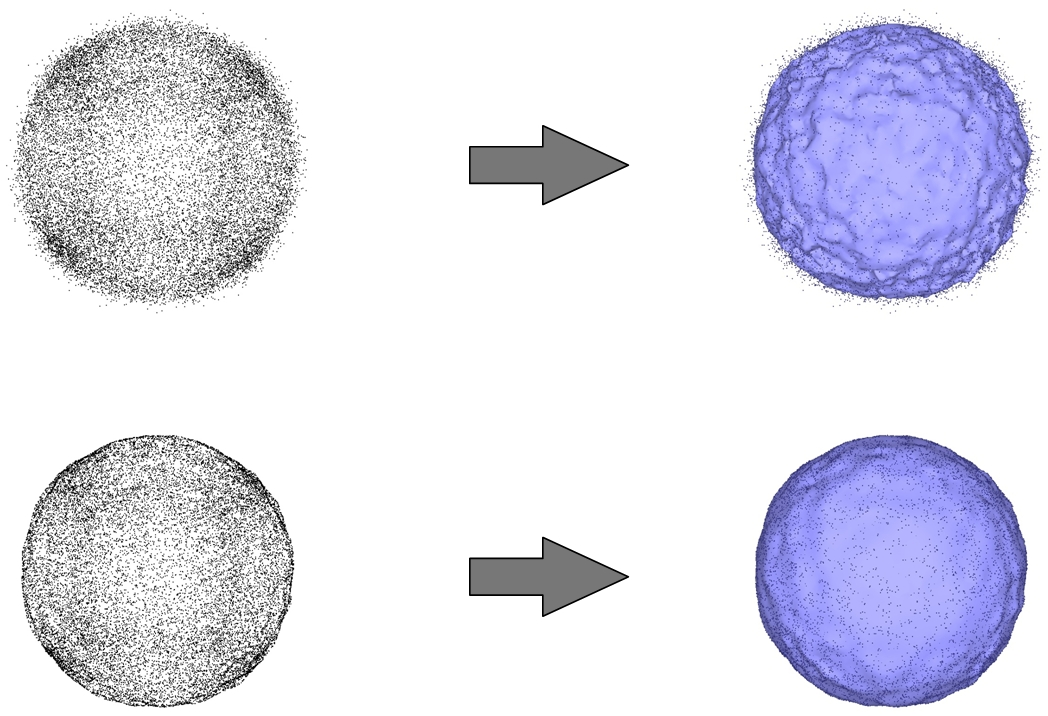
\includegraphics[width=0.8\textwidth]{Surface_reconstruction_points_3/noise}
    \end{ccTexOnly}
    \begin{ccHtmlOnly}
        <img style="max-width: 80%;" border=0 src="./noise.jpg"><P>
    \end{ccHtmlOnly}
    \begin{figure}[h]
        \caption{Top-left: points sampled on a sphere and corrupted with a
                 lot of noise.
                 Top-right: reconstructed surface mesh.
                 Bottom-left: smoothed point set.
                 Bottom-right: reconstructed surface mesh.}
        \label{Surface_reconstruction_points_3-fig-noise}
    \end{figure}
\end{center}

For a large number of outliers the failure cases (not shown) translate into spurious small connected components and massive distortion near the inferred surface. In this case the outliers must be removed through \ccc{CGAL::remove_outliers()}.


\subsubsection{Sharp Creases}

The current reconstruction algorithm is not able to recover the sharp creases and corners present in the inferred surface. This translates into smoothed sharp creases.

% Insert image sharp_features.jpg/.eps
\begin{center}
    \begin{ccTexOnly}
        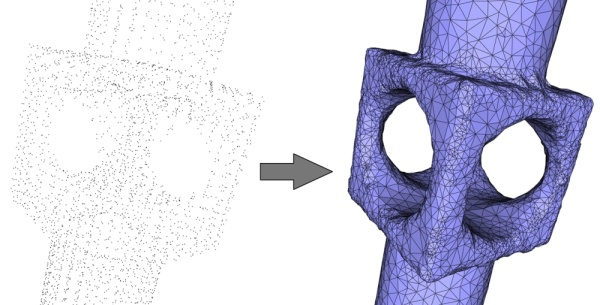
\includegraphics[width=0.8\textwidth]{Surface_reconstruction_points_3/sharp_features}
    \end{ccTexOnly}
    \begin{ccHtmlOnly}
        <img style="max-width: 80%;" border=0 src="./sharp_features.jpg"><P>
    \end{ccHtmlOnly}
    \begin{figure}[h]
        \caption{Left: 5K points sampled on a mechanical piece with
                 sharp features (creases, darts and corners).
                 Right: reconstructed surface mesh with smoothed
                 creases.}
        \label{Surface_reconstruction_points_3-fig-sharp_features}
    \end{figure}
\end{center}

